\section{Limiti} \label{sec_limiti}
Prendiamo una successione abbastanza semplice da definire, tipo:
\begin{equation*}
    a_n = \frac{n-1}{n}
\end{equation*}
Cominciamo ora ad elencare i suoi termini e calcoliamo i suoi valori:
\begin{align*}
    a_1 &= \dfrac{0}{1} = 0\\
    a_2 &= \dfrac{1}{2} = 0.5\\
    a_3 &= \dfrac{2}{3} = 0.\overline{6}\\
    a_4 &= \dfrac{3}{4} = 0.75\\
    \vdots\\
    a_{1000} &= \dfrac{999}{1000} = 0.999\\
    \vdots\\
    a_{100000} &= \dfrac{99999}{100000} = 0.99999\\
\end{align*}
È facile notare che più $n$ diventa grande più il valore della successione 
\textit{tende} a $1$. Come si formalizza questa cosa? Con il concetto di 
limite.

\subsection{Limite di una successione} \label{sec_lim_successioni}
\dfn{
    Data una successione $(a)_n$, e un numero $L \in \mathbb{R}$, si dice che 
    $(a)_n$ è \textbf{convergente} e si indica:
    \begin{equation*}
        \lim_{n \to +\infty} a_n = L \qquad \text{oppure} \qquad (a)_n 
        \xrightarrow[n \to +\infty]{} L
    \end{equation*}
    \qquad se
    \begin{equation*}
        \forall \epsilon > 0, \exists \bar{n} = \bar{n}(\epsilon) \in 
        \mathbb{N}: \forall n \geq \bar{n}: |a_n - L| < \epsilon
    \end{equation*}
}

\dfn{
    Data una successione $(a)_n$, si dice che $(a)_n$ è \textbf{divergente} e 
    si indica:
    \begin{itemize}
        \item \begin{equation*}
                \lim_{n \to +\infty} a_n = +\infty \qquad \text{oppure} \qquad 
                (a)_n \xrightarrow[n \to +\infty]{} +\infty
            \end{equation*}
            \qquad se
            \begin{equation*}
                \forall \epsilon > 0, \exists \bar{n} = \bar{n}(\epsilon) \in 
                \mathbb{N}: \forall n \geq \bar{n}: a_n \geq \epsilon
            \end{equation*}
        \item \begin{equation*}
                \lim_{n \to +\infty} a_n = -\infty \qquad \text{oppure} \qquad 
                (a)_n \xrightarrow[n \to +\infty]{} -\infty
            \end{equation*}
            \qquad se
            \begin{equation*}
                \forall \epsilon > 0, \exists \bar{n} = \bar{n}(\epsilon) \in 
                \mathbb{N}: \forall n \geq \bar{n}: a_n \leq -\epsilon
            \end{equation*}
    \end{itemize}
}

\imp{
    \begin{center}
        Se esiste il limite di una successione esso è \textbf{unico}
    \end{center}
}

Esistono successioni che non hanno limite (non sono né convergenti né 
divergenti).
\begin{gather*}
    a_n = (-1)^2\\
    a_0 = 1,\; a_1 = -1,\; a_2 = 1 \;\cdots
\end{gather*}
La successione è limitata in quanto i suoi valori sono $-1 e 1$, eppure non ha 
limite in quanto oscilla.
\begin{gather*}
    a_n = (-1)^n \cdot n\\
    a_0 = 0,\; a_1 = -1,\; a_2 = 2,\; a_3 = -3,\; a_4 = 4 \;\cdots
\end{gather*}
La successione in quanto caso non è limitata e non ha un limite in quanto 
"salta" tra valori positivi e valori negativi.

\subsection{Numero di Eulero (o Nepero)} \label{sec_numeroDiEulero}
Prendiamo in considerazione la serie
\begin{equation*}
    a_n = \left(1+\dfrac{1}{n} \right)^n
\end{equation*}
Dimostriamo che è una serie \textbf{convergente}, e chiamiamo il suo limite 
\textbf{\textit{e}}. Quindi:
\begin{equation*}
    \lim_{n\to +\infty} \left(1+\dfrac{1}{n}\right)^n = e \in \mathbb{R}
\end{equation*}

\mlem{
	È necessario, per questa dimostrazione, introdurre la 
    \textit{disuguaglianza di Bernoulli}. 
	\begin{equation*}
		\forall x \in \mathbb{R} : x \geq -1, \forall n \in \mathbb{N}: 
        (1+x)^n \geq 1 + nx
	\end{equation*}

    Dimostrazione: proviamo la disuguaglianza di Bernoulli per induzione. 
	\begin{enumerate}
		\item Caso $n = 1$:
			\begin{align*}
				(1+x)^1 &\geq 1 + 1 \cdot x\\[5pt]
				1 + x &\geq 1 + x
			\end{align*}

		\item Caso $n+1$:
			Ipotesi induttiva sappiamo che vale $(1+x)^n \geq 1 + nx$.
			Dimostriamo che:
			\begin{align*}
				(1+x)^{n+1} \geq 1 + (n+1)x
			\end{align*}
			Considerando solo la parte sinistra:
			\begin{align*}
				(1+x)^{n+1} = (1+x)^n \cdot (1+x)
			\end{align*}
			Usando l'ipotesi induttiva:
			\begin{align*}
				(1+x)^n \cdot (1+x) &\geq (1+nx) \cdot (1+x) = 1 + x + nx + 
                nx^2\\
				&= 1 + (n+1) \cdot x + nx^2
			\end{align*}
			Quindi:
			\begin{equation*}
				(1+x)^{n+1} \geq 1 + (n+1) \cdot x + nx^2
			\end{equation*}
			Ed essendo $nx^2 \geq 0$ si può togliere in quanto non cambierebbe 
            la disequazione:
			\begin{equation*}
				(1+x)^{n+1} \geq 1 + (n+1) \cdot x
			\end{equation*}
	\end{enumerate}
	\hfill Qed.
}

Facciamo ora la dimostrazione riguardante il numero di Eulero:

\pf{
    Per dimostrare che una successione è convergente ci basta dimostrare che è 
    (strettamente) crescente e limitata. Questo dal corollario della 
    dimostrazione nella sezione \ref{corol_successioni}.
    \begin{enumerate}
        \item Dimostriamo che $(a_n)$ è (strettamente) crescente:
            Per dimostrare che $(a_n)_n \nearrow$ ci basta dimostrare che:
            \begin{equation*}
                \dfrac{a_{n+1}}{a_n} > 1 \qquad \forall n
            \end{equation*}
            \begin{align*}
                \dfrac{a_{n+1}}{a_n} &= \dfrac{\left(1+\dfrac{1}{n+1}\right)^{n+1}}
                {\left(1+\dfrac{1}{n}\right)^n} = \dfrac{\left(\dfrac{n+2}{n+1}
                \right)^{n+1}}{\left(\dfrac{n+1}{n}\right)^n}
                = \dfrac{\dfrac{n+2}{n+1} \cdot \left( \dfrac{n+2}{n+1} 
                \right)^n}{\left(\dfrac{n+1}{n}\right)^n} =\\[5pt]
                &= \dfrac{n+2}{n+1} \cdot \left( \dfrac{n+2}{n+1} \cdot 
                \dfrac{n}{n+1} \right)^n = \dfrac{n+2}{n+1} \cdot \left( 
                \dfrac{n^2+2n+1-1}{n^2+2n+1} \right)^n =\\[5pt]
                &= \dfrac{n+2}{n+1} \cdot \left( 1 -\dfrac{1}{n^2+2n+1} 
                \right)^n = \dfrac{n+2}{n+1} \cdot \left( 1 + \left( 
                -\dfrac{1}{n^2+2n+1}\right) \right)^n
            \end{align*}
            Usiamo la disuguaglianza di Bernoulli. Però assicuriamoci prima di 
            poterla usare:
            \begin{gather*}
                x = - \dfrac{1}{n^2+2n+1} \geq -1\\
                \dfrac{1}{n^2+2n+1} \leq 1\\
                1 \leq n^2+2n+1\\
                0 \leq n^2+2n
            \end{gather*}
            Verificato! Ora usiamola:
            \begin{align*}
                &\dfrac{n+2}{n+1} \cdot \left( 1 + \left( 
                -\dfrac{1}{n^2+2n+1}\right) \right)^n \geq \dfrac{n+2}{n+1} 
                \cdot \left( 1 + n\left( -\dfrac{1}{n^2+2n+1}\right) 
                \right)=\\[5pt]
                &= \dfrac{n+2}{n+1} \cdot \dfrac{n^2+2n+1-n}{n^2+2n+1} = 
                \dfrac{n+2}{n+1} \cdot \dfrac{n^2+n+1}{n^2+2n+1} =\\[5pt]
                & = \dfrac{n^3+3n^2+3n+1+1}{n^3+3n^2+3n+1} = 1 + 
                \dfrac{1}{n^3+3n^2+3n+1} > 1
            \end{align*}

        \item Dobbiamo provare ora che $(a_n)_n$ è limitata. Usiamo il binomio 
            di newton:
            \begin{align*}
                (1+\dfrac{1}{n})^n &= \sum_{k = 0}^{n} \binom{n}{k} \cdot 
                1^{n-k} \cdot \left(\dfrac{1}{n}\right)^k = \sum_{k = 0}^{n} 
                \binom{n}{k}\dfrac{1}{n^k} = \sum_{k = 0}^{n} 
                \dfrac{n!}{(n-k)!k!}\cdot\dfrac{1}{n^k}=\\
                &= \sum_{k = 0}^{n} \dfrac{n \cdot (n-1) \cdots (n-k+1)}{n^k} 
                \cdot \dfrac{1}{k!} =\\
                &= \sum_{k = 0}^{n} \dfrac{n}{n} \cdot \dfrac{(n-1)}{n} \cdots 
                \dfrac{(n-k+1)}{n} \cdot \dfrac{1}{k!} =
            \end{align*}
            È facile notare che:
            \begin{equation*}
                \dfrac{n}{n} \cdot \dfrac{(n-1)}{n} \cdots \dfrac{(n-k+1)}{n} 
                \leq 1
            \end{equation*}
            In quanto il denominatore sarà sempre più grande del numeratore 
            (tranne per il primo termine) e quindi ogni singolo termine sarà 
            $\leq 1$ ed essendo tutti moltiplicati tra di loro il risultato 
            sarà anch'esso $\leq 1$. Possiamo quindi concludere che:
            \begin{equation*}
                = \sum_{k = 0}^{n} \dfrac{n}{n} \cdot \dfrac{(n-1)}{n} \cdots 
                \dfrac{(n-k+1)}{n} \cdot \dfrac{1}{k!} \leq \sum_{k = 0}^{n} 
                \dfrac{1}{k!} = 2 + \sum_{k = 2}^{n} \dfrac{1}{k!}
            \end{equation*}
            Possiamo notare che:
            \begin{equation*}
                k! = k\cdot (k-1)\cdot (k-2) \cdots 1 \geq k (k-1) > 0 \qquad 
                \text{per } k\geq 2
            \end{equation*}
            \begin{equation*}
                \implies k! > k(k-1) \implies \dfrac{1}{k!} < \dfrac{1}{k(k-1)} 
                = \dfrac{1}{k-1} - \dfrac{1}{k}
            \end{equation*}
            Quindi sostituendo
            \begin{align*}
                &< 2 + \sum_{k = 0}^{n} \left(\dfrac{1}{k-1} - 
                \dfrac{1}{k}\right) = 2 + \left[ \left(1-\dfrac{1}{2}\right) + 
                \left(\dfrac{1}{2}-\dfrac{1}{3}\right) + \left(\dfrac{1}{3}-
                \dfrac{1}{4}\right) \cdots \left(\dfrac{1}{n-1}-\dfrac{1}{n}
                \right)\right]=
            \end{align*}
            Le coppie di termini dentro la parentesi quadre condividono il 
            primo elemento con il secondo della coppia precedente. Se si 
            espandono le somme si cancellano tutti tranne il primo e l'ultimo:
            \begin{equation*}
                = 2 + \left[1 - \dfrac{1}{n}\right] = 3 -\dfrac{1}{n} < 3
            \end{equation*}
            Quindi:
            \begin{equation*}
                a_n = \left(1+\dfrac{1}{n}\right)^{n} < 3 \qquad \forall n \in 
                \mathbb{N}
            \end{equation*}
            Dunque $(a_n)_n \nearrow$ è superiormente limitata. Ne consegue 
            che, dal corollario presente nella sezione \ref{corol_successioni}:
            \begin{equation*}
                \exists \lim_{n\to + \infty} \left(1+\dfrac{1}{n}\right)^n = e
            \end{equation*}
    \end{enumerate}
    \hfill Qed.
}
Si può dimostrare che $e \notin \mathbb{Q}$, quindi è un numero irrazionale e 
il suo valore è approssimativamente:
\begin{equation*}
    e \approx 2,71828 18284 59045 23536 \cdots
\end{equation*}

\subsection{Limite di una funzione}

\dfn{
\textbf{Intorno sferico di un punto} $x_0 \in \mathbb{R}$ di raggio $r$:
    \begin{equation*}
        x_0 \in \mathbb{R}, r\in \mathbb{R} : r > 0
    \end{equation*}
    \begin{equation*}
        I_r (x_o) = \left\{x\in \mathbb{R} : \; |x-x_0| < r \right\}
    \end{equation*}
    Che in pratica risulta:
    \begin{equation*}
        I_r (x_0) = ]x_0-r, x_0+r[
    \end{equation*}
}

\dfn{
    $x_0$ si dice \textbf{punto di accumulazione} di $\mathbb{A} \subseteq 
    \mathbb{R}$ se:
    \begin{equation*}
        \forall r > 0: A\cap \left( I_r (x_0) \setminus \{x_0\} \right) \neq 
        \emptyset
    \end{equation*}
}
Comunque prendo piccolo $r$ c'è sempre un elemento di $\mathbb{A}$ diverso da 
$x_0$. L'insieme dei punti di accumulazione di un insieme è indicato come 
segue\footnote{La lettera che indica l'insieme dei punti di accumulazione è una 
"D" che dovrebbe essere celtica. Fate riferimento agli appunti del prof in 
questo caso perché non riesco a trovare su \LaTeX\; il simbolo esatto che usa 
lui. Il fatto è che ci si può confondere perché si usa la lettera "D" anche per 
indicare il dominio di una funzione. In questi appunti il dominio è indicato 
con $Dom()$ mentre l'insieme dei punti di accumulazione è indicato con 
$\mathcal{D}$.}:
\begin{equation*}
	\mathcal{D} (\mathbb{A}) = \left\{ x \in \mathbb{R}\; |\; x\; \text{è un 
    punto di accumulazione di}\; \mathbb{A} \right\}
\end{equation*}
Posso in pratica avvicinarmi indefinitamente ad $x_0$ sempre rimanendo in 
$\mathbb{A}$

\textbf{Proposizione:}\\
$\mathbb{A} \subseteq \mathbb{R}, x_o \in \mathbb{R}$. $x_0$ è un punto di 
accumulazione per A se e solo se $\exists (a_n)_n \subseteq \mathbb{A}$ t.c.
\begin{enumerate}
	\item $a_n \neq x_0 \quad \forall n \in \mathbb{N}$
	\item $a_n \xrightarrow[n\to +\infty]{} x_0$
\end{enumerate}
Esempio:
$\mathbb{A} = \left\{\dfrac{1}{n} \;\middle|\; n \in \mathbb{N} \setminus \{0\} 
\right\}$
\begin{equation*}
    \lim_{x\to + \infty} \dfrac{1}{x} = 0 \implies \mathcal{D}(\mathbb{A}) = {0}
\end{equation*}

Un insieme con $\mathcal{D} = \emptyset $ è un \textbf{insieme discreto}

\subsection{Limite destro e limite sinistro}
Se si vuole indicare il limite per $x \to x_0$ di una funzione $f(x)$ si 
indica:
\begin{equation*}
	\lim_{x \to x_0} f(x)
\end{equation*}
\textbf{Questo limite esiste solo se sono rispettate le seguenti condizioni:}
\begin{equation*}
	\exists \lim_{x \to x_0} f(x) = l \in \mathbb{R} \cup \{+\infty\} \cup 
    \{-\infty\}\iff 
	\begin{cases*}
		\exists \lim_{x \to x_o^-} f(x)\\
		\exists \lim_{x \to x_o^+} f(x)\\
		\lim_{x \to x_0^-} f(x) = \lim_{x \to x_0^+} = l \in \mathbb{R} \cup 
        \{+\infty\} \cup \{-\infty\}
	\end{cases*}
\end{equation*}
In pratica il limite destro e sinistro devono esistere e il loro valore deve 
coincidere.

Se ci avviciniamo da destra (cioè da valori più grandi) ad un punto $x_0$ si 
scrive che $x_0^+$, se invece ci avviciniamo da sinistra (cioè da valori più 
piccoli) si scrive $x_0^-$.

\subsubsection{SCHEMA RIASSUNTIVO LIMITI:} 
Per tradurre un limite nella notazione epsilon-delta il seguente schema può 
tornare effettivamente molto utile.
\begin{equation*}
	\lim_{\cdots} f(x) = \cdots
\end{equation*}

Nella parte inferiore del limite i casi sono i seguenti:
\begin{enumerate}[label=(\roman*)]
    \item $x\to x_0$
    \item $x\to x_0^+$
    \item $x\to x_0^-$
    \item $x\to +\infty$
    \item $x\to -\infty$
\end{enumerate}

Mentre per la parte destra dell'uguale i casi sono i seguenti:
\begin{enumerate}
    \item $l \in \mathbb{R}$
    \item $+ \infty$
    \item $- \infty$
\end{enumerate}

\textbf{Tradotto}:
\begin{equation*}
    \forall \epsilon >0, \exists \delta > 0: \forall x \in \mathcal{D}(f) :
    \begin{cases*}
        0 < |x-x_0| < \delta \qquad \text{(i)}\\
        x_0 < x < x_0 + \delta \qquad \text{(ii)}\\
        x_0 - \delta < x < x_0 \qquad \text{(iii)}\\
        x > \delta \qquad \qquad\qquad\;\; \text{(iv)}\\
        x < - \delta \qquad \qquad\qquad \text{(v)}
    \end{cases*}
    \qquad
    \implies 
    \begin{cases*}
        |f(x) - l| < \epsilon \qquad 1\\
        f(x) > \epsilon \qquad\qquad\, 2\\
        f(x) < \epsilon \qquad\qquad\, 3
    \end{cases*}
\end{equation*}

Quindi se per esempio devo tradurre il seguente limite:
\begin{equation*}
	\lim_{x \to 5^-} f(x) = +\infty
\end{equation*}
Vedo che $x \to 5^-$ è l'opzione numero (iii), mentre a destra dell'uguale 
($+\infty$) ho l'opzione 2. Quindi diventa:
\begin{equation*}
	\forall \epsilon > 0, \exists \delta > 0 : \forall x \in \mathcal{D}(f): 5 
    - \delta < x < 5 \implies f(x) > \epsilon
\end{equation*}

\subsection{Algebra dei limiti}
L'algebra dei limiti vale sia per le successioni che per le funzioni. Per 
comodità in seguito è riportata con il caso delle funzioni:\\
Siano $f(x)$ e $g(x)$ due funzioni tale che
\begin{equation*}
    f(x) \xrightarrow{\qquad} l_1 \qquad g(x) \xrightarrow{\qquad} l_2
\end{equation*}
Allora:
\begin{equation*}
    f(x)+g(x) \xrightarrow{\qquad}
    \begin{cases*}
        l_1 + l_2 \qquad \text{se}\;\;\, l_1,l_2 \in \mathbb{R}\\
        +\infty \quad\, \qquad \text{se}\;\;\, l_1 = +\infty \land (l_2 \in 
        \mathbb{R} \lor l_2 = +\infty)\\
        -\infty \quad\, \qquad \text{se}\;\;\, l_1 = -\infty \land (l_2 \in 
        \mathbb{R} \lor l_2 = -\infty)\\
        \text{Stessa cosa se si scambia $l_1$ con $l_2$}
    \end{cases*}
\end{equation*}

\begin{equation*}
    f(x) \cdot g(x) \xrightarrow{\qquad}
    \begin{cases*}
        l_1 \cdot l_2 \qquad \text{se}\;\;\, l_1,l_2 \in \mathbb{R}\\
        +\infty \quad\, \qquad \text{se}\;\;\, l_1 = +\infty \land (l_2 \in 
        \mathbb{R}_+^* \lor l_2 = +\infty)\\
        +\infty \quad\, \qquad \text{se}\;\;\, l_1 = -\infty \land (l_2 \in 
        \mathbb{R}_-^* \lor l_2 = -\infty)\\
        -\infty \quad\, \qquad \text{se}\;\;\, l_1 = +\infty \land (l_2 \in 
        \mathbb{R}_-^* \lor l_2 =-\infty)\\
        -\infty \quad\, \qquad \text{se}\;\;\, l_1 = -\infty \land (l_2 \in 
        \mathbb{R}_+^* \lor l_2 = +\infty)\\
        \text{Stessa cosa se si scambia $l_1$ con $l_2$}
    \end{cases*}
\end{equation*}
con $g(x) \neq 0$
\begin{equation*}
    \dfrac{f(x)}{g(x)} \xrightarrow{\qquad}
    \begin{cases*}
        \dfrac{l_1}{l_2} \qquad \text{se}\;\;\, l_1,l_2 \in \mathbb{R}\\
        0 \quad\, \qquad \text{se}\;\;\, l_1 \in \mathbb{R} \land l_2 = \pm \infty\\
        \pm \infty \quad\, \qquad \text{se}\;\;\, l_1 = \pm \infty \land l_2 
        \in \mathbb{R}_+^*\\
        \mp \infty \quad\, \qquad \text{se}\;\;\, l_1 = \pm \infty \land l_2 
        \in \mathbb{R}_-^*\\
        \text{Stessa cosa se si scambia $l_1$ con $l_2$}
    \end{cases*}
\end{equation*}

\subsubsection{Forme indeterminate}
Non essendo presenti tutti i casi nell'algebra dei limiti nascono quelle che 
vengono chiamate \textbf{forme indeterminate} in quanto corrispondo a 
situazione non univoche dove il risultato non si può stabilire a priori, ma è 
necessario trattare ogni caso singolarmente. Di seguito una lista di queste 
forme:
\begin{itemize}
    \item $+\infty - \infty$
    \item $-\infty + \infty$
    \item $0 \cdot \pm \infty $
    \item $\dfrac{\pm \infty}{\pm \infty}$
    \item $\dfrac{0}{0}$
\end{itemize}

\textbf{NOTA}: Le espressioni che contengono i simboli $+\infty$ e $-\infty$ 
sono solo \textbf{espressioni formali}, non hanno alcun valore matematico!

\subsection{Teoremi dei limiti}
\thm{ \label{theorem_permanenzaSegno}
Teorema di \textbf{permanenza del segno}. Data $f: A \to \mathbb{R}$, $x_0 \in 
\mathcal{D}(A)$ e
\begin{equation*}
    \lim_{x \to x_0} f(x) = l \in \mathbb{R} \;\; \land \;\; l > 0
\end{equation*}
Allora:
\begin{equation*}
    \exists \delta > 0: \forall x \in A, x_0 - \delta < x < x_0 + \delta, x 
    \neq x_0 \implies f(x) > 0
\end{equation*}
Vale anche nel caso di $l < 0$.
}

\thm{\label{theorem_confronto}
Teorema del \textbf{confronto}. $f, g, h: A \to \mathbb{R}$, $x_0 \in 
\mathcal{D}(A)$ e 
\begin{equation*}
    \lim_{x \to x_0} g(x) = \lim_{x \to x_0} h(x) = l \in \mathbb{R}
\end{equation*}
\begin{equation*}
    \exists \epsilon > 0: g(x) \leq f(x) \leq h(x), \forall x \in \left[ A\cup 
    I_r(x_0) \right] \setminus {x_0} \implies \lim_{x \to x_0} f(x) = l
\end{equation*}
}

\thm{ %Ma che teorema è questo??
	Aiuta i calcoli con le forme indeterminate $\dfrac{k}{0}$ con $k \neq 0$. 
    Data una funzione $f:A \to \mathbb{R}$ e un punto $x_0 \in \mathcal{A}$. 
    $\exists \delta > 0$:
	\begin{enumerate}
		\item Sx: 
			\begin{equation*}
				f(x) > 0 \quad \forall x \in A : x_0 - \delta < x < x_0
			\end{equation*}
			Quindi:
			\begin{equation*}
				\lim_{x \to x_0^-} f(x) = 0^{+}
			\end{equation*}
			Allora:
			\begin{equation*}
				\lim_{x \to x_0^-} \dfrac{1}{f(x)} = + \infty
			\end{equation*}

			Se $f < 0$ allora $0^-$ e $-\infty$.

		\item Dx:
			\begin{equation*}
				f(x) > 0 \quad \forall x \in A : x_0 < x < x_0 + \delta
			\end{equation*}
			Quindi:
			\begin{equation*}
				\lim_{x \to x_0^+} f(x) = 0^{+}
			\end{equation*}
			Allora:
			\begin{equation*}
				\lim_{x \to x_0^+} \dfrac{1}{f(x)} = + \infty
			\end{equation*}

			Se $f < 0$ allora $0^-$ e $-\infty$.

	\end{enumerate}
}

\subsection{Limiti Notevoli} \label{sec_limitiNotevoli}
I limiti notevoli sono particolari limiti che nonostante siano una forma 
indeterminata, il loro valore è conosciuto. In realtà molti limiti con forme 
indeterminate hanno un valore conosciuto perché attraverso tecniche e metodi di 
calcolo si riesce a ricavare. La differenza con i limiti notevoli però è che 
questi ultimi sono estremamente fondamentali per molte dimostrazioni e per 
molti esercizi. Inoltre comprendono solo funzioni elementari e vengono 
dimostrati una volta per tutte e poi vengono dati per buoni nel calcolo dei 
limiti.\\
Il limite notevole più famoso e sicuramente più importante è:
\imp{
\begin{equation*}
    \lim _{x\to 0} \dfrac{\sin{x}}{x} = 1
\end{equation*}
}
Per dimostrarlo è prima necessario dimostrare 2 lemmi:
\mlem{
Dobbiamo dimostrare:
\begin{equation*}
    \lim_{x \to 0} \sin{x} = 0
\end{equation*}
Costruiamo una circonferenza goniometrica come in figura:
\begin{center}


	\def\tmpval{0.7071067812}

	\begin{tikzpicture}[scale=3]

	\draw (0,0) circle (1cm);

	\begin{scope}
		\draw[->] (-1.5,0) -- (1.5,0) node[right] {$x$};
		\draw[->] (0,-1.5) -- (0,1.5) node[above] {$y$};
	\end{scope}

	\filldraw[fill=green!20] (0,0) -- (3mm,0pt) arc(0:45:3mm);
		\draw (15:2mm) node {$x$};

	\draw[-] (0,0) -- (\tmpval,\tmpval);
	\draw[-] (0,0) -- (\tmpval,-\tmpval);
	\draw[-] (\tmpval,0) -- (\tmpval,\tmpval);
	\draw[-] (\tmpval,0) -- (\tmpval,-\tmpval);

	\draw[very thin, fill] (\tmpval,\tmpval) circle (0.4pt) node[right, 
        yshift=5pt] {$P$};
	\draw[very thin, fill] (\tmpval,0) circle (0.4pt) node[right, 
        yshift=5pt] {$H$};
	\draw[very thin, fill] (\tmpval,-\tmpval) circle (0.4pt) node[right, 
        yshift=-5pt] {$P'$};



	\draw[very thin, fill] (1,0) circle (0.4pt) node[right, yshift=10pt] {$A$};
	\draw[very thin, fill] (0,0) circle (0.4pt) node[left, yshift=10pt] 
        {$(0, 0)$};


\end{tikzpicture}

\end{center}



Per la definizione di seno e coseno: $\sin{x} = \overline{HP}$ e $\cos{x} = 
\overline{OH}$. Inoltre $\overline{PP'} < \arc{PP'}$ perché il "percorso" più 
breve tra due punti in geometria euclidea è il segmento che li congiunge. 
Facendo qualche semplificazione:
\begin{align*}
    \overline{PP'} &< \arc{PP'}\\
    2\overline{HP} &< 2\arc{PA}\\
    \overline{HP} &< \arc{PA}
\end{align*}
Essendo segmenti, ed essendo quindi sempre positivi, riscriviamo la nostra 
disuguaglianza con il valore assoluto.
\begin{equation*}
    \left | \overline{HP} \right | < \left | \arc{PA} \right |
\end{equation*}
Si noti che per la precedente definizione di seno, per la definizione di angolo 
in radianti e per il fatto che siamo sulla circonferenza goniometrica che ha 
raggio pari a 1:
\begin{equation*}
    \left | \sin{x} \right | < \left | x \right |
\end{equation*}
Ed essendo il valore assoluto sempre maggiore o uguale a zero:
\begin{equation*}
    0 \leq \left | \sin{x} \right | < \left | x \right |
\end{equation*}
Dal teorema del confronto (Sezione: \ref{theorem_confronto}) si ha che:
\begin{equation*}
    \lim _{x \to 0} \left | \sin{x} \right | = 0
\end{equation*}
e quindi:
\begin{equation*}
    \lim _{x \to 0} \sin{x} = 0
\end{equation*}
\hfill Qed.
}
\mlem{
Dobbiamo dimostrare:
\begin{equation*}
    \lim_{x \to 0} \cos{x} = 1
\end{equation*}
Facciamo qualche trasformazione algebrica e usiamo la duplicazione del coseno 
(Sezione: \ref{sec_formuleDuplicazione}):
\begin{equation*}
    \cos{x} = \cos \left ( 2 \cdot \dfrac{x}{2} \right ) = 1 - 2\sin^2 
    \left(\dfrac{x}{2} \right)
\end{equation*}
Ne consegue che:
\begin{equation*}
    1 - \cos{x} = 2\sin^2 \left(\dfrac{x}{2} \right)
\end{equation*}
Dal lemma precedente abbiamo:
\begin{align*}
    0 \leq \left | \sin{x} \right | &< \left | x \right |\\
    0 \leq \left | \sin \left( \dfrac{x}{2}\right) \right | &< \left | 
    \dfrac{x}{2} \right |\\
    0 \leq \sin^2 \left( \dfrac{x}{2}\right) &< \dfrac{x^2}{4}\\
    0 \leq 2\sin^2 \left( \dfrac{x}{2}\right) &< \dfrac{x^2}{2}
\end{align*}
E quindi facendo una sostituzione:
\begin{equation*}
    0 \leq 1 - \cos{x} = 2\sin^2 \left( \dfrac{x}{2} \right) < \dfrac{x^2}{2}
\end{equation*}
Sempre per il teorema del confronto (in quanto $x \to 0$ implica $\frac{x^2}{2} 
\to 0$):
\begin{equation*}
    \lim_{x \to 0} 2\sin^2 \left( \dfrac{x}{2} \right) = 0
\end{equation*}
Sostituendo:
\begin{equation*}
    \lim_{x \to 0} 1 - \cos{x} = 0
\end{equation*}
E quindi:
\begin{equation*}
    \lim_{x \to 0} \cos{x} = 1
\end{equation*}
\hfill Qed.
}
Finito di dimostrare i lemmi passiamo ora a dimostrare il limite notevole vero 
e proprio:
\pf{
Dobbiamo dimostrare:
\begin{equation*}
    \lim_{x \to 0} \dfrac{\sin{x}}{x} = 1
\end{equation*}
Disegniamo un arco di circonferenza goniometrica (quindi con centro 
nell'origine e raggio 1). Il segmento $\overline{AH}$ è perpendicolare a 
$\overline{OB}$. Il segmento $\overline{AD}$ è perpendicolare a 
$\overline{AC}$.

\begin{center}


	\def\cosval{0.5}
	\def\sinval{0.8660254038}
	\def\tanval{\sinval / \cosval}
	\def\xval{0.640718}
	\def\yval{0.900251}
	

	\begin{tikzpicture}[scale=3]

	\draw (0,0) circle (1cm);

	\begin{scope}
		\draw[->] (-2,0) -- (2,0) node[right] {$x$};
		\draw[->] (0,-2) -- (0,2) node[above] {$y$};
	\end{scope}

	\filldraw[fill=green!20] (0,0) -- (3mm,0pt) arc(0:60:3mm);
		\draw (15:2mm) node {$x$};

	\draw[-] (0,0) -- (1, \tanval);
	\draw[-] (\cosval,0) -- (\cosval,\sinval);
	\draw[-] (\cosval,\sinval) -- (1, 1 / \sinval -\cosval / \sinval);
	\draw[->] (1,0) -- (1,2);


	\draw[-] (\cosval * 1.1, \sinval * 1.1) -- (\xval, \yval);
	\draw[-] (0.5907186, 0.8136489) -- (\xval, \yval);

	\draw[very thin, fill] (\cosval,\sinval) circle (0.4pt) node[left, 
        xshift=5pt, yshift=10pt] {$A$};
	\draw[very thin, fill] (\cosval,0) circle (0.4pt) node[right, 
        yshift=5pt] {$H$};
	\draw[very thin, fill] (1,0) circle (0.4pt) node[right, 
        yshift=10pt] {$B$};
	\draw[very thin, fill] (1,\tanval) circle (0.4pt) node[right] {$C$};
	\draw[very thin, fill] (1, 1 / \sinval - \cosval / \sinval) circle (0.4pt) 
        node[right] {$D$};
	\draw[very thin, fill] (0,0) circle (0.4pt) node[left, yshift=10pt] 
        {$(0, 0)$};


\end{tikzpicture}

\end{center}

Assumiamo per iniziare $0 < x < \dfrac{\pi}{2}$. Per definizione di seno, 
coseno e tangente abbiamo che:
\begin{itemize}
    \item $A(\cos{x}, \sin{x})$
    \item $B(1, 0)$
    \item $C(1, \tan{x})$
\end{itemize}

Notiamo che $\overline{AH} \leq \arc{AB}$ in quanto $\overline{AB} \leq 
\arc{AB}$, per il fatto che la distanza tra due punti in geometria euclidea è 
il segmento che li congiunge, e $\overline{AH} \leq \overline{AB}$ in quanto 
$ABH$ è un triangolo rettangolo dove $\overline{AB}$ è l'ipotenusa.\\

Dobbiamo inoltre notare che $\arc{AB} \leq \overline{BC}$, in quanto $\arc{AB} 
< \overline{BD} + \overline{AD}$ dalla geometria euclidea, inoltre 
$\overline{BD} + \overline{AD} < \overline{BD} + \overline{DC}$ in quanto 
$\overline{AD}$ è un cateto del triangolo $ACD$ dove $\overline{CD}$ è 
l'ipotenusa. Basta infine notare che $\overline{BD} + \overline{DC} = 
\overline{BC}$ e quindi:
\begin{equation*}
    \overline{AH} \leq \arc{AB} \leq \overline{BC}
\end{equation*}
Essendo
\begin{equation*}
    \sin{x} = \overline{AH} \qquad x = \arc{AB} \qquad \tan{x} = \overline{BC}
\end{equation*}
sostituendo diventa:
\begin{equation*}
    \sin{x} \leq x \leq \tan{x}
\end{equation*}
Visto che all'inizio abbiamo posto la condizione $0 < x < \dfrac{\pi}{2}$, per 
forza $\sin{x} > 0$. Possiamo quindi dividere tutto per $\sin{x}$:
\begin{equation*}
    \dfrac{\sin{x}}{\sin{x}} \leq \dfrac{x}{\sin{x}} \leq \dfrac{\tan{x}}
    {\sin{x}} = \dfrac{\sin{x}}{\cos{x}} \cdot \dfrac{1}{\sin{x}} = 
    \dfrac{1}{\cos{x}}
\end{equation*}
Sia $\frac{x}{\sin{x}}$, sia $\frac{1}{\cos{x}}$ sono maggiori di zero per $0 < 
x < \frac{\pi}{2}$. Possiamo quindi passare ai reciproci:
\begin{equation*}
    1 \geq \dfrac{\sin{x}}{x} \geq \cos{x} \qquad \left( 0 < x < \dfrac{\pi}{2} 
    \right)
\end{equation*}
In realtà, essendo $\sin{x}$ una funzione dispari e $\cos{x}$ una funzione 
pari:
\begin{equation*}
    \dfrac{\sin(-x)}{-x} = \dfrac{-\sin{x}}{-x} = \dfrac{\sin{x}}{x}
\end{equation*}
\begin{equation*}
    \cos(-x) = \cos x
\end{equation*}
Questo vuol dire che la relazione scritta sopra vale anche per l'intervallo 
negativo $-\dfrac{\pi}{2} < x < 0$. Quindi:
\begin{equation*}
    1 \geq \dfrac{\sin{x}}{x} \geq \cos{x} \qquad \left( 0 < |x| < 
    \dfrac{\pi}{2} \right)
\end{equation*}
Per il lemma dimostrato precedentemente che prova che $\lim_{x \to 0} \cos{x} 
= 1$ e il teorema del confronto (Sezione: \ref{theorem_confronto}):
\begin{equation*}
    \lim_{x \to 0} = \dfrac{\sin{x}}{x} = 1
\end{equation*}
\hfill Qed.
}
Da questo teorema è possibile dimostrare l'area della circonferenza. Se infatti 
prendiamo una circonferenza generica $C$ di raggio $r$ e ci inscriviamo un 
poligono regolare $S_n$ di $n$ lati (come in figura \ref{fig_cfrPoligon}):
\begin{equation*}
	\mathcal{A}(\mathcal{C}) = \lim_{n \to + \infty} \mathcal{A} (S_n)
\end{equation*}
In questo caso $\mathcal{A}$ rappresenta l'area. Osserviamo che:
\begin{equation*}
	\alpha = \dfrac{2\pi}{n} \implies \dfrac{a}{2}= \dfrac{\pi}{n}
\end{equation*}
Inoltre usando un po' di trigonometria:
\begin{align*}
	\overline{OH_1} &= \overline{OA_1} \cdot \cos \left( \dfrac{\alpha}{2}
    \right) = r \cdot \cos \left(\dfrac{\pi}{n}\right)\\[5pt]
	\overline{A_1H_1} &= \overline{OA_1} \cdot \sin \left( \dfrac{\alpha}{2}
    \right) = r \cdot \sin \left(\dfrac{\pi}{n}\right)
\end{align*}
Quindi:
Ne consegue che:
\begin{equation*}
	\mathcal{A} (\stackrel{\triangle}{OA_1A_2}) = 2 \cdot \mathcal{A} 
    (\stackrel{\triangle}{OA_1H}) = \overline{A_1H} \cdot \overline{OH} = r^2 
    \cdot \sin \left(\dfrac{\pi}{n} \right) \cdot \cos \left(\dfrac{\pi}{n} 
    \right)
\end{equation*}

L'area di tutto il poligono quindi risulta:
\begin{equation*}
	\mathcal{A} (S_n) = n \cdot \mathcal{A} (\stackrel{\triangle}{OA_1A_2}) = 
    n \cdot r^2 \cdot \sin \left(\dfrac{\pi}{n} \right) \cdot \cos 
    \left(\dfrac{\pi}{n} \right)
\end{equation*}

Ora se calcoliamo il limite:
\begin{equation*}
	\lim_{n \to + \infty} \mathcal{A}(s_n) = \lim_{n \to + \infty} n \cdot r^2 
    \cdot \sin \left(\dfrac{\pi}{n} \right) \cdot \cos \left(\dfrac{\pi}{n} 
    \right) = \lim_{n \to + \infty} r^2 \cdot \pi \cdot \dfrac{\sin 
    \left(\dfrac{\pi}{n} \right)}{\dfrac{\pi}{n}} \cdot \cos \left(\dfrac{\pi}
    {n} \right)
\end{equation*}
Facendo un piccolo cambio di variabile:
\begin{equation*}
	m := \dfrac{\pi}{n} \qquad m \xrightarrow[n \to +\infty]{} 0
\end{equation*}
Quindi:
\begin{equation*}
	\lim_{m \to 0} r^2 \cdot \pi \cdot \dfrac{\sin(m)}{m} \cdot \cos (m) =  r^2 
    \cdot \pi \cdot 1 \cdot 1
\end{equation*}
Ne consegue che l'area della circonferenza:
\begin{equation*}
	\mathcal{A}(\mathcal{C}) = \lim_{n \to + \infty} \mathcal{A} (S_n) = \pi 
    \cdot r^2
\end{equation*}

\begin{figure}
\begin{center}
	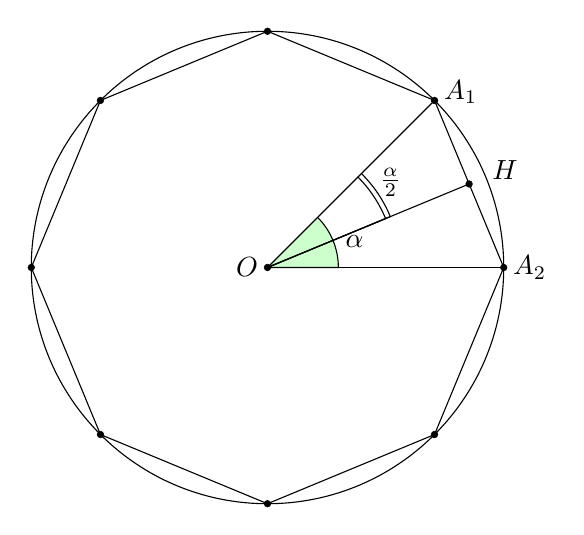
\begin{tikzpicture}[scale=3]

	\def\tmpval{0.707106}

	\draw (0,0) circle (1cm);

	\filldraw[fill=green!20] (0,0) -- (3mm,0pt) arc(0:45:3mm);
		\draw (15:2mm) node[xshift=15pt, yshift=5pt] {$\alpha$};

	\draw[] (0,0) -- (0.5, 0.2071) arc(22.5:45:5.45mm);
	\draw[] (0,0) -- (0.52, 0.4142135 * 0.52) arc(22.5:45:5.57mm) node[right, 
        xshift=3pt, yshift=-3pt] {$\frac{\alpha}{2}$};

	\draw[-] (0,0) -- (\tmpval, \tmpval);
	\draw[-] (0,0) -- (1, 0);
	\draw[-] (0,0) -- (0.8535539, 0.35355339);


	\draw[-] (1,0) -- (\tmpval, \tmpval);
	\draw[-] (\tmpval, \tmpval) -- (0, 1);
	\draw[-] (\tmpval, -\tmpval) -- (0, -1);
	\draw[-] (1,0) -- (\tmpval, -\tmpval);

	\draw[-] (0, 1) -- (-\tmpval, \tmpval);
	\draw[-] (-\tmpval, \tmpval) -- (-1, 0);
	\draw[-] (-\tmpval, -\tmpval) -- (-1, 0);
	\draw[-] (0,-1) -- (-\tmpval, -\tmpval);



	\draw[very thin, fill] (0,0) circle (0.4pt) node[left] {$O$};
	\draw[very thin, fill] (1,0) circle (0.4pt) node[right] {$A_2$};
	\draw[very thin, fill] (0.8535539, 0.35355339) circle (0.4pt) node[right, 
        xshift=5pt, yshift=5pt] {$H$};
	\draw[very thin, fill] (\tmpval,\tmpval) circle (0.4pt) node[right, 
        yshift=3pt] {$A_1$};
	\draw[very thin, fill] (0,1) circle (0.4pt);
	\draw[very thin, fill] (-\tmpval,\tmpval) circle (0.4pt);
	\draw[very thin, fill] (-1,0) circle (0.4pt);
	\draw[very thin, fill] (-\tmpval,-\tmpval) circle (0.4pt);
	\draw[very thin, fill] (0,-1) circle (0.4pt);
	\draw[very thin, fill] (\tmpval,-\tmpval) circle (0.4pt);


\end{tikzpicture}
	\end{center}
	\caption{Circonferenza con inscritto un poligono regolare di $n$ lati}
	\label{fig_cfrPoligon}
\end{figure}

Un secondo limite notevole:
\imp{
\begin{equation*}
    \lim_{x \to 0} \dfrac{1 - \cos{x}}{x^2} = \dfrac{1}{2}
\end{equation*}
}
\pf{
\begin{align*}
    &\lim_{x \to 0} \dfrac{1 - \cos{x}}{x^2} = \lim_{x \to 0} 
    \dfrac{1-\cos^2{x}}{x^2} \cdot \dfrac{1}{1 + \cos{x}} =\\
    =&\lim_{x \to 0} \dfrac{\sin^2{x}}{x^2} \cdot \dfrac{1}{1 + \cos{x}} = 
    \lim_{x \to 0} \left( \dfrac{\sin{x}}{x} \right)^2 \cdot \dfrac{1}{1 + 
    \cos{x}} = \\
    =&\lim_{x \to 0} \left( \dfrac{\sin{x}}{x} \right)^2 \cdot \lim_{x \to 0} 
    \dfrac{1}{1 + \cos{x}} = 1 + \dfrac{1}{2} = \dfrac{1}{2}
\end{align*}
}

Un terzo limite notevole che deriva dal secondo:
\imp{
\begin{equation*}
    \lim_{x \to 0} \dfrac{1 - \cos{x}}{x} = 0
\end{equation*}
}

\pf{
\begin{equation*}
    \lim_{x \to 0} \dfrac{1 - \cos{x}}{x} = \lim_{x \to 0} \dfrac{1 - 
    \cos{x}}{x^2} \cdot x = \dfrac{1}{2} \cdot 0 = 0
\end{equation*}
}
Altri limiti notevoli:
\imp{
\begin{equation*}
    \lim_{x \to 0} \dfrac{a^x-1}{x} = \ln{a} \qquad (0 < a,\;\; a \neq 1)
\end{equation*}
}

Il caso particolare in qui $a = e$:
\imp{
\begin{equation*}
    \lim_{x \to 0} \dfrac{e^x-1}{x} = 1
\end{equation*}
}

\subsection{Asintoti}
\dfn{
$x = k$ è un \textbf{asintoto verticale} per $f(x)$ se
\begin{equation*}
    \lim_{x\to k^{+}} f(x) = \pm \infty \qquad \text{oppure} \qquad \lim_{x\to 
    k^{-}} f(x) = \pm \infty
\end{equation*}
}
Ne consegue che graficamente l'asintoto verticale si verifica quando la 
funzione sotto esame tende a $\pm \infty$ in un punto specifico (come in figura 
\ref{fig_asintotVer}):

\begin{figure}[h]
\begin{center}
	\begin{tikzpicture}
	\begin{axis}[xmax = 4, xmin = -0.5, ymax = 10, ymin = -10,
		axis lines=middle, xlabel=$x$, ylabel=$y$, ylabel style={anchor=east}, 
        xlabel style={anchor=north},
		     ytick style={draw=none},
		     yticklabels={},
		     xtick={2},
		     xticklabels={$k$},
		     xticklabel style={anchor=north west},
		    ]
		\addplot[samples=800]{1/(x-2) + 3 * x - 5};
	\end{axis}
	\end{tikzpicture}

\end{center}
	\caption{Asinto veritcale}
	\label{fig_asintotVer}
\end{figure}


\dfn{
$y = l$ si dice \textbf{asintoto orizzontale} se: $f: A\to \mathbb{R}$, 
$\sup A = +\infty$ e 
\begin{equation*}
    \lim_{x\to + \infty} f(x) = l \in \mathbb{R}
\end{equation*}
Vale ovviamente anche il caso a $-\infty$. Nella stessa funzione ci possono 
essere al massimo 2 asintoti orizzontali.
}

\begin{figure}[h]
\begin{center}
	\begin{tikzpicture}
	\begin{axis}[xmax = 4, xmin = -2, ymax = 10, ymin = -10,
		axis lines=middle, xlabel=$x$, ylabel=$y$, ylabel style={anchor=east}, 
        xlabel style={anchor=north},
		     yticklabel style={anchor=north east},
		     ytick={-3},
		     yticklabels={$l$},
		     xticklabel style={draw=none},
		    ]
		\addplot[samples=800]{e^(-1.5* x) - 3};
		\addplot[samples=800]{-3};
	\end{axis}
	\end{tikzpicture}

\end{center}
	\caption{Asinto orizzontale}
\end{figure}

\subsection{Limiti di funzioni elementari}
IL limite di un polinomio $p(x)$ è il polinomio calcolato nel punto:
\begin{equation*}
    \lim_{x \to x_0} p(x) = p(x_0)
\end{equation*}
\pf{
Dimostriamo che il limite di un polinomio $p(x)$ è il polinomio calcolato nel 
punto:
\begin{equation*}
    \lim_{x \to x_0} p(x) = p(x_0)
\end{equation*}
dove $x_0 \in \mathbb{R}$. Partiamo dal caso base:
\begin{equation*}
    \lim_{x \to x_0} x = x_0
\end{equation*}
Questo deriva direttamente dalla definizione di limite con $\delta = \epsilon$. 
Ora dall'algebra dei limiti:
\begin{align*}
    &\lim_{x \to x_0} x^2 = \lim_{x \to x_0} x \cdot \lim_{x \to x_0} x = 
    x_0^2\\
    &\lim_{x \to x_0} x^3 = \lim_{x \to x_0} x^2 \cdot \lim_{x \to x_0} x = 
    x_0^3\\
    & \qquad \qquad \vdots \\
    &\lim_{x \to x_0} x^j = x_0^j \qquad (j \in \mathbb{R} )\\
\end{align*}
Se aggiungiamo un coefficiente ($a \in \mathbb{R}$) davanti al polinomio non 
cambia nulla, infatti:
\begin{equation*}
    \lim_{x \to x_0} ax^j = \lim_{x \to x_0} a \cdot \lim_{x \to x_0} x_0^j = 
    a x_0^j
\end{equation*}
Possiamo quindi provare una importante proprietà dei polinomi. Dato infatti un 
polinomio generico di grado $n$:
\begin{equation*}
    p(x) = \sum _{i = 0}^n a_i \cdot x^i
\end{equation*}
Vale che quello che vogliamo dimostrare, infatti:
\begin{equation*}
    \lim_{x \to x_0} \sum _{i = 0}^n a_i \cdot x^i = \sum _{i = 0}^n \lim_{x 
    \to x_0} a_i \cdot x^i = \sum _{i = 0}^n a_i \cdot x_0^i = p(x_0)
\end{equation*}
\hfill Qed.
}

Di seguito un elenco di limiti delle funzioni elementari. Alcuni sono 
abbastanza ovvi quindi non ci sono dimostrazioni allegate:

\begin{multicols}{2}
    \begin{equation*}
        \lim _{x \to +\infty} \ln(x) = +\infty
    \end{equation*}
    
    \begin{equation*}
        \lim _{x \to 0^+} \ln(x) = -\infty
    \end{equation*}
    
    \begin{equation*}
        \lim _{x \to +\infty} e^x = +\infty
    \end{equation*}

    \begin{equation*}
        \lim _{x \to -\infty} e^x = 0^+
    \end{equation*}

    \begin{equation*}
        \lim _{x \to +\infty} \sqrt{x} = +\infty
    \end{equation*}

    \begin{equation*}
        \lim _{x \to 0^+} \sqrt{x} = 0^+
    \end{equation*}

    \begin{equation*}
        \not \exists \lim _{x \to \pm \infty} \sin{x}
    \end{equation*}
    
    \begin{equation*}
        \not \exists \lim _{x \to \pm \infty} \cos{x}
    \end{equation*}
\end{multicols}

%NE MANCA QUALCUNA?

\subsection{Confronto di infiniti} \label{sec_gerarchiaInfiniti}

Se si hanno due funzioni che vanno a $+\infty$ si possono confrontare. Il 
confronto ci permette di determinare qualche delle due funzioni "\textit{va a 
infinito più velocemente}". Si riesce quindi a stilare una sorta di "gerarchia" 
degli infiniti dove alcuni tendono a $+\infty$ più velocemente di altri. Questo 
è molto utile negli esercizi e soprattutto in analisi della complessità 
computazionale.\\

Date quindi due funzioni $f(x)$ e $g(x)$ che tendono entrambe a $+ \infty$ se:
\begin{equation*}
    \lim \dfrac{f(x)}{g(x)} =
    \begin{cases*}
        0 \qquad \qquad g \text{ cresce più velocemente di } f\\
        +\infty \qquad \;\;\; f \text{ cresce più velocemente di } g\\
        l \neq 0 \qquad \; \text{$f$ e $g$ sono infinitesimi dello stesso 
        ordine}
    \end{cases*}
\end{equation*}
Non vi è qui riportata la dimostrazione in quanto necessita di un teorema visto 
più avanti. Per completezza la dimostrazione è comunque riportata nella sezione 
\ref{dim_gerarchiaInfiniti}, subito dopo il teorema in questione. La decisione 
di riportare questa gerarchia qui è che ha molto senso con i limiti nonostante 
non si possa ancora dimostrare. La gerarchia degli infiniti risulta (dal più 
"lento" al più "veloce"):
\begin{enumerate}
	\item $\log_a^m (x)$ con $a > 1$ e $m \in \mathbb{N}$
	\item $p(x)$
	\item $a^x$ con $a > 1$
	\item $x^x$
\end{enumerate}
Ne consegue quindi che, per esempio, $x^{100^{100^{100}}}$ è "più lento" di 
$(1,000001)^x$, cioè che:
\begin{equation*}
    \lim_{x \to + \infty} \dfrac{x^{100^{100^{100}}}}{(1,000001)^x} = 0
\end{equation*}

\subsection{Continuità di una funzione}
\dfn{
$x_0 \in A$ si dice \textbf{punto isolato di} $A\subseteq \mathbb{R}$ se $x_o 
\not \in \mathcal{D}(A)$. In pratica se non è un punto di accumulazione
}
\dfn{
Una funzione $f: A \to \mathbb{R}$ si dice \textbf{continua} in $x_0 \in A$ se:
\begin{enumerate}
    \item $x_0 \not \in \mathcal{D}(A)$ (cioè $x_0$ è un punto isolato di $A$)
    \item $x_0 \in \mathcal{D}(A) \implies \lim \limits_{x\to x_0} f(x) = 
        f(x_0)$
\end{enumerate}
(Si noti che le due opzioni non possono valere contemporaneamente, sono quindi 
congiunte da un \textit{or} invece che un \textit{and}).
}
Se $f:A \to \mathbb{R}$ è continua $\forall x \in A$. allora è continua su $A$. 
Si scrive
\begin{equation*}
    f \in \mathcal{C} (A)
\end{equation*}
dove $\mathcal{C}(A)$ è l'insieme delle funzioni continue su $A$, ed è definito 
come:
\begin{equation*}
    \mathcal{C}(A) = \{ f:A\to \mathbb{R}\; |\; f\; \text{è continua in x}, 
    \forall x \in A \}
\end{equation*}
La continuità è un grado molto importante per "classificare" la regolarità di 
una funzione. Inoltre moltissimi teoremi che riguardano una o più funzioni 
richiedono che queste siano continue. L'idea che ci sta dietro alla continuità 
e il voler classificare rigorosamente tutte quelle funzioni "belle" che puoi 
disegnare senza staccare la mano dal foglio\footnote{In realtà non è esattamente 
così, però è un buon modo per iniziare a capire l'argomento}.\\
Come vi diranno tutti i professori di analisi però, la definizione di 
continuità che si basa sul disegnare una funzione senza staccare la mano dal 
foglio è sbagliata. Questo perché vale solo per quelle funzioni che sono 
continue su tutto $\mathbb{R}$, mentre per quelle che sono continue nel loro 
dominio, ma proprio questo dominio è composto dall'unione di molteplici 
intervalli disgiunti, allora restano continue, ma per disegnarle è necessario 
comunque staccare la mano dal foglio.

\dfn{
Il \textbf{dominio naturale} è il più grande sottoinsieme in cui una funzione è 
definita
}

Dai teoremi di algebra dei limiti segue che date due funzioni $f: A \to 
\mathbb{R}$ e $g: B \to \mathbb{R}$ continue in $x_0 \in A \cap B$ allora:
\begin{multicols}{2}
    \begin{itemize}
        \item $f \pm g$ è continua in $x_0$
        \item $c \in \mathbb{R}$ : $c\cdot f$ è continua in $x_0$
        \item $f \cdot g$ è continua in $x_0$
        \item $\dfrac{f}{g}$ è continua in $x_0$ (se $g(x_0) \neq 0$)
        \item $|f|$ è continua in $x_0$
        \item $g(f(x_0))$ è continua in $x_0$ se $x_0 \in A \land f(x_0) \in B$ 
            e $f$ è continua in $x_0$ e $g$ è continua in $f(x_0)$
    \end{itemize}
\end{multicols}

\pf{
Dimostriamo che $|x|$ è una funzione continua.
\begin{equation*}
    f(x) = |x| =
    \begin{cases*}
        x \quad \;\;\, \text{se} \quad x \geq 0\\
        -x \quad \text{se} \quad x < 0
    \end{cases*}
\end{equation*}
Prendiamo un punto $x_0 \in \mathbb{R}$, abbiamo due casi:
\begin{itemize}
    \item Caso $x_0 \neq 0$:
        \begin{equation*}
            \lim_{x \to x_0} |x| =
            \begin{cases*}
                \text{se} \quad x_0 > 0: \lim_{x \to x_0} |x| = \lim_{x \to 
                x_0} x = x_0 = |x_0|\\
                \\
                \text{se} \quad x_0 < 0: \lim_{x \to x_0} |x| = \lim_{x \to 
                x_0} -x = -x_0 = |x_0|
            \end{cases*}
        \end{equation*}

    \item Caso $x_0 = 0$:
        \begin{align*}
            &\lim_{x \to 0^-} |x| = \lim_{x \to x^-} -x = 0\\
            &\lim_{x \to 0^+} |x| = \lim_{x \to x^+} x = 0
        \end{align*}
        Questo implica che:
        \begin{equation*}
            \lim_{x \to 0} |x| = 0 = |0|
        \end{equation*}
\end{itemize}
E quindi dalla definizione di continuità, $|x|$ è una funzione continua su 
tutto $\mathbb{R}$.
\hfill Qed.
}

\pf{
Dimostriamo che $\sin(x)$ è una funzione continua. In pratica dobbiamo provare 
che
\begin{equation*}
    \lim_{x \to x_0} \sin(x) = \sin(x_0) \qquad (\forall x_0 \in \mathbb{R})
\end{equation*}
Possiamo riscrivere $\sin(x)$ come $\sin (x_0 + (x - x_0))$. Chiamiamo $h$ il 
fattore $h :=(x-x_0)$. Quando $x \to x_0$, $h \to 0$. Quindi possiamo 
riscrivere il limite da dimostrare nel seguente modo:
\begin{equation*}
    \lim_{x \to h} \sin(x_0 + h) = \sin(x_0) \qquad (\forall x_0 \in \mathbb{R})
\end{equation*}
Avendo riscritto l'argomento del seno attraverso una somma, possiamo applicare 
le formule di addizione del seno:
\begin{equation*}
    \sin(x_0 + h) = \sin(x_0)\cos(h) + \sin(h)\cos(x_0)
\end{equation*}
Sostituendo quindi nel limite (in quanto per $h \to 0$, $\cos(h) \to 1$ e 
$\sin(h) \to 0$):
\begin{equation*}
    \lim_{x \to h} \sin(x_0 + h) =  \lim_{x \to h} \sin(x_0)\cos(h) + 
    \sin(h)\cos(x_0) = \sin(x_0)
\end{equation*}
\hfill Qed.
}
\pf{
Dimostriamo che $\cos(x)$ è una funzione continua. In pratica dobbiamo provare 
che
\begin{equation*}
    \lim_{x \to x_0} \cos(x) = \cos(x_0) \qquad (\forall x_0 \in \mathbb{R})
\end{equation*}
Con lo stesso trucco usato nella dimostrazione precedente ci riduciamo 
dimostrare:
\begin{equation*}
     \lim_{x \to h} \cos(x_0 + h) = \cos(x_0) \qquad (\forall x_0 \in 
     \mathbb{R})
\end{equation*}
Usando le formule di addizione del coseno:
\begin{equation*}
    \cos(x_0 + h) = \cos(x_0)\cos(h) - \sin(x_0)\sin(h)
\end{equation*}
Sostituiamo nel limite e calcoliamo (in quanto per $h \to 0$, $\sin(h) \to 0$ e 
$\cos(h) \to 1$):
\begin{equation*}
    \lim_{x \to h} \cos(x_0 + h) = \lim_{x \to h} \cos(x_0)\cos(h) - 
    \sin(x_0)\sin(h) = \cos(x_0)
\end{equation*}
\hfill Qed.
}

La \textbf{continuità della tangente} nel suo dominio naturale è dovuta dal 
fatto che la tangente può essere definita come rapporto tra \textit{seno} e 
\textit{coseno}, e il rapporto di funzioni continue è anch'esso continuo. 
L'\textbf{esponenziale} è continuo. Tutte le \textbf{funzioni inverse delle 
funzioni elementari} sono continue ($\ln{x}$, $\sqrt{x}$, $\arcsin{x}$, 
$\arccos{x}$ e $\arctan{x}$).\\

\subsubsection{Funzioni definite a tratti}
Per le funzioni definite a tratti il caso è un po' più particolare perché non 
si sa a priori se sono continue o no. In generale il metodo per scoprire se 
sono continue è il seguente. Prendiamo una funzione $f$ definita a tratti in 
questo modo:
\begin{equation*}
    f(x) =
    \begin{cases*}
        g(x) \qquad (x \leq a)\\
        h(x) \qquad (x > a)
    \end{cases*}
\end{equation*}
Di solito sia $g$ che $h$ sono funzioni formate da composizioni di funzioni 
elementari, che rendono automaticamente continue le due funzioni. Il problema 
sorge quindi nel punto di separazione $a$. Per verificare che sia continua la 
funzione $f$ bisogna fare in modo che sia $g$ sia $h$ si avvicinino ad $a$ con 
lo stesso valore, cioè che abbiano lo stesso limite per $x \to a$.
\begin{equation*}
    \lim_{x \to a^-} g(x) = \lim_{x \to a^+} h(x)
\end{equation*}
Inoltre è richiesto che il limite coincida con il valore della funzione $f(a)$. 
In questo caso non abbiamo fatto il test perché il valore della funzione era 
compreso nella funzione $g$ in quanto era definito per $\leq$ invece che un 
minore stretto. Se però questo non fosse il caso va inserito $f(a)$ nelle 
uguaglianze dei limiti scritti sopra.
